%%%%%%%%%%%%%%%%%%%%%%%%%%%%%%%%%%%%%%%%%%%%%%%%%%%%%%%%%%%
% Chapter1


\pagestyle{fancy} 
\chapter{Background}
\label{cha:1}
\vspace{1cm}

\section{Variational Auto-Encoder (VAE) Structure}
Before starting to talk about the usage VAEs, it is mandatory to go through the structure of the auto-encoder which is essentially a neural network with a bottleneck in the middle Fig~\ref{fig:autoencoder} designed to reconstruct the original input in an unsupervised way, in other words, it learns an identity function by first reducing the dimension of the data to the bottleneck so as to extract more efficient and compressed representation. Surprisingly The idea was originated in the 1980s, and later promoted by the seminal paper by~\cite{hinton2006reducing}.

\vspace{0.3cm}
The Auto-Encoder consists of tow connected networks that could be any kind of neural networks (convolutional, or multi-layer perceptron etc) depends on the data it has to deal with, which are:
\begin{itemize}
	\item Encoder network: gets the high-dimension input and transform it to into a low-dimension code in the bottleneck, or we can call it representation, latent or features as well again depends on what the usage are we making of the auto-encoder.
	\item Decoder network: gets the output of the encoder and does essentially the inverse process, or we can say reconstruct the data, likely with larger and larger layers to the last one that outputs the reconstructed original data.
\end{itemize}

\begin{figure}
	\centerline
	\autoencoder
	\caption{Autoencoder}
	\label{fig:autoencoder}
\end{figure} 

We can see already how the auto-encoder networks can give us an efficient way to  impressively represent the data and in lower dimension. So the accomplishment of solutions for the problematics we talked about at beginning of this session, is all about about how we build the bottleneck layer or what will call from now on vector $z$. The VAE~\cite{kingma2013auto} basically is an auto-encoder but the structure of vector $z$ is quite different. For instance what if we need to map the input into a probability distribution $q_{\theta}$ instead of a fixed vector $z$, where $q_{\theta}$ is parameterized by $\theta$, from which we sample or generate $z$, this is what make the VAE to be recognized as a generative model. Where the training is regularized to avoid eventual overfitting  that might occur with auto-encoder architecture and ensure that the distribution $q_{\theta}$ has good parameters to enable the generative process. The way that makes the encoder to be able to produce $q_\theta$ is by composing the bottleneck or the output of a mean $\mu$ and a covariance matrix $\Sigma$ the problem here is that nothing would prevent the this distribution to be extremely narrow, or effectively a single value. To escape the issue, the Kullback–Leibler (KL) divergence-which measures the distance between tow distributions- is introduced  between the distribution produced by the encoder $q_{\theta}(z \mid x_i)$ and a unit Gaussian distribution $p(z)$(mean $0$, covariance matrix is the identity matrix) and tell us how much information is lost when using q to represent p, this KL divergence is then introduced as a penalty to the loss function li, which consists of another term as well that is the expected negative likelihood of the $i$-th datapoint $x_i$ as follow:


\begin{equation}
l_i(\theta,\phi)=-E_{z\sim q_\theta (z\mid x_i)}[\log_{p_\phi}(x_i \mid z)]+KL(q_\theta (z\mid x_i)||p(z))
\label{eq:VAE_loss}
\end{equation}
Where $z$ is sampled from $q_\theta$ and $\phi$ the decoder parameters, the purpose of the first term in poor words mean “how much the decoder output is similar to original datapoint $x_i$“. It intuitively leads the decoder to learn to reconstruct the data. The last important part left to talk about is the training one, we can use the gradient descent to optimize the loss with respect to the parameters of the encoder and decoder $\theta$ and $\phi$ respectively. For stochastic gradient descent with step size $\rho$, the encoder parameters are updated using $\theta=\theta-\frac{\partial l}{\partial \theta} $  and the decoder is updated similarly.



\subsection{Reparameterization Trick:}
As we can notice at this point that there would be a problem doing the backpropagation step of the gradient descent optimizer, because it does not go through the random node z, therefore we have to implement some trick to circumvent this issue. The reparameterization trick~\cite{kingma2013auto} is essentially done by introducing an auxiliary variable (noise) $\varepsilon$ that allows us to reparameterize $z$ in a way that allows backpropagate to flow through the deterministic nodes as shown in Fig.~\ref{fig:paratrick}, we are basically expressing the random variable $z$ as a deterministic 

\begin{figure}
	\centerline
	\paratrick
	\caption{reparameterization trick}
	\label{fig:paratrick}
\end{figure} 

\section{Gaussian Mixture Models (GMMs) structure and learning algorithm}
The model is parameterized by two types of values, the mixture component weights are defined as ϕk and the component means μk and variances σk or covariances (for the multivariant case) Σ, the mixture component weights has a constraint that is:  $\sum_{i=1}^{K} \phi_i = 1$ so that the total probability distribution normalizes to 1. The numerical technique used to maximize the likelihood estimation is the “Estimation maximization (EM)” which consists of tow steps:

\begin{itemize}
	\item	 E-step: consist of calculating the the expectation of the component assignments $P(C_k | x_i)$ for each data point $x_i \in X$ given the model parameters $\phi_k$,  $\mu_k$, and $\sigma_k$.
\end{itemize}
\begin{itemize}
	\item	M-step: which consists of maximizing the expectations calculated in the E step with respect to the model parameters. This step consists of updating the values $\phi_k$,  $\mu_k$, and $\sigma_k$.
\end{itemize}
The entire process iteratively repeats until the algorithm converges, before it starts some initializations are made as follows:
Randomly assign samples without replacement from the dataset $X={x_1, ..., x_N}$, to the component mean estimates $\mu_1, … , \mu_k$. E.g. for K=3 and N=100, set $\mu_1= x_45$, $\mu_2 = x_32$, $\mu_3 = x_10$. 
Set all component variance estimates to the sample variance 
$\sigma_1^2,...,\sigma_k^2=\frac{1}{N}\sum_{i=1}^{K} (x_i -\hat{x})^{2}=1$, where $\hat{x}=\frac{1}{N}\sum_{i=1}^{N}(x_i)$ is the sample mean.
Set all component distribution prior estimates to the uniform distribution  
$P(C_k) = \phi_1,..., \phi_k  = \frac{1}{K}$
while the E-step computes the probability that $x_i$ is generated by component $C_k$:
\begin{equation}
p(C_j \mid x_i ) = \frac{ p(x_i \mid C_j)p(C_j) }{p(x_i)} = \frac{p(x_i \mid C_j)p(C_j)}{\sum_ip(x_i \mid C_j)p(C_j)}
\label{eq:}	
\end{equation}

which will be used in the M-step where the parameters are updated as follow:	

\begin{align}
\mu_j&=\frac{ \sum_{i} p(C_j \mid x_i )x_i}{\sum_{i} {p(C_j \mid x_i )}} \\
\sigma_j^2 &=\frac{\sum_{i}{p ( C_j \mid x_i)}  (x_i - \mu_j) (x_i - \mu_j)^T} {\sum_{i} {p(C_j \mid x_i )}} \\
p ( C_j ) &= \frac{ \sum_{i} p(C_j \mid x_i )}{N}
\end{align}

\begin{figure}
	\centering
	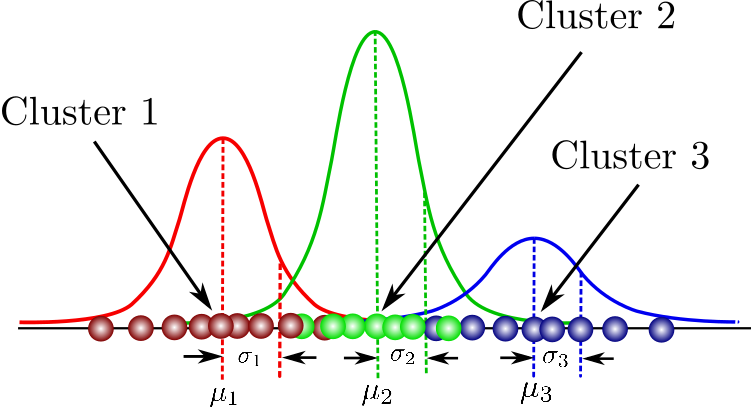
\includegraphics[scale=0.3]{Figures/GMM}
	\caption{}
	\label{fig:GMM}
\end{figure}

\vspace{10pt} 
Originally GMM is employed for classification and clustering tasks, but as we can deduce that it is also a suitable model when recovering the distribution of the data is needed, since it can produce more complexed distribution composed of jointed k gaussians as in Fig.~\ref{fig:GMM}, for example if we have different sources from which the data is provided. Back to our main argument, GMM has been used in several robotics applications, like in Gaussian Mixture Model for Robotic Policy Imitation~\cite{pignat2019bayesian} where different robots had to learn from few amount of demonstrations to complete various tasks such as avoid obstacles, or insert a peg in a moving hole. This approach (GMM) illustrates the advantages of learning a distribution of policies instead of trajectories and can be used in a variety of tasks. On the other hand in some work as in~\cite{zhang2016robot} the GMM was benefited in robot obstacle avoidance learning as a base for a generative model, to generate trajectories, by Gaussian Mixture Regression (GMR), The trajectory obtained not only can avoid obstacles but also can be executed by robots due to its good smooth property. The same idea of~\cite{zhang2016robot} was implemented in~\cite{reiley2010motion} in which GMM encodes the expert’s underlying motion structure. GMR is then used to extract a smooth reference trajectory to reproduce a trajectory of the task. This GMM/GMR generative model was trained on expert data, then tested by classifying the generated trajectories  to be either coming from expert, intermediate, or novice surgeons. The classification algorithm Hidden Markov Models (HMMs) trains three (expert, intermediate and novice) from five new unseen trials for each skill level. The results of the classifier show that each trajectories generated by GMM/GMR are closest to the expert model. To conclude this session it is right and proper to say that the use of GMM has remarkable impact to improve the model performance in presence of lack of data issue.


%\vspace{1cm}
\section{Employment of VAEs in generative models for robotics}
\label{sec:VAE_generative}
Lets go now through some papers to see where and how the VAEs have been employed and show their effectiveness in various applications of generative models in robotics. The first one~\cite{eslami2016attend} where a framework called by the authors "Attend, infer, repeat" (AIR) the VAE structure here is quite different that the encoder was implemented as a Recurrent Neural Network (RNN), since its purpose is to learn to detect and generate objects, specifically “where is the objects, what are they and how many are they”. The additional recurrence to the structure is basically to detect how many objects are present in the input data. Experiments were designed initially on 2D data particularly on multiple MNIST digits, and reliably the model were able to detect and generate the constituent digits from scratch, it shows advantages over state-of-art generative models computationally and also in terms of generalization to unseen datasets. Other Experiments on 3D datasets, considering scenes consisting of only one of three objects: a red cube, a blue sphere, and a textured cylinder. The network accurately and reliably infers the identity and pose of the object, on the other hand, an identical network trained to predict the ground-truth identity and pose values of the training data has much more difficulty in accurately determining the cube’s orientation.\\

Moreover, in robotics, grasping and manipulation of various objects is a critical and challenging problem,~\cite{veres2017modeling} has proposed another concept referred to as the grasp motor image (GMI) that combines object perception and a learned prior over grasp configurations, to synthesize new grasps to apply to a different object. At the core of GMI is the autoencoder structure, taking advantage of Deep  Learning (DL), particularly building both encoder and decoder as Convolutional Neural Networks (CNN). The approach followed is intuitive: based on
perceptual information about an object, and an idea of how an object was previously grasped, collecting a object/grasp pair dataset of successful, cylindrical precision robotic grasps using the V-REP  simulator~\cite{rohmer2013v}, and object files provided by~\cite{kleinhans2015g3db} on a simulated “picking” task. The VAE was trained on this dataset to generate grasps for novel objects. GMI integrates
perceptual information and grasp configurations using deep generative models. Applying it to a simulated grasping task, has demonstrated the capacity of these models to transfer learned knowledge to novel objects under varying amounts of available training data.\\

\chapter{Reinforcement Learning (RL)}
\label{cha:3}
\vspace{1cm}

\section{What is RL}
This field of machine learning deals with how an agent ought to behave in an environment in order to maximize the reward. It differs from supervised learning in not needing of labeled input/output pairs and from unsupervised learning in getting guidance from the environment by performing actions and learning from the errors or rewards. Typically the environment take the form of a Markov Decision Process (MDP) is a mathematical system used for modeling decision making. We use a tuple (S, A, P, R, $\gamma$) to define a MDP. Where S denotes the state space, a finite set of states. A denotes a set of actions the actor can take at each time step t. P denotes the probability that taking action a at time step t in state st will result in state $s_{t+1}$. $R_a(s,\acute{s})$ is the expected reward from taking action a and transitioning to $\acute{s}$. $\gamma \in [0, 1]$ is a discount factor, to discount the future reward.

\vspace{0.3cm}
There are tow notions about the environment where the algorithm that implement RL that should be mentioned which are:
\begin{itemize}
	\item “model-based” algorithms: who are employed when the environment is a priori known, in other words, when we know the transition probability matrix P between states, so the agent can make predictions about the next state and reward before it takes each action.
\end{itemize}
\begin{itemize}
	\item “model-free” algorithms: for which there is no assumption about the world.
\end{itemize}
While about the techniques the algorithm uses to lean the policy are divided as follow:
\begin{itemize}
	\item \textquotedblleft Off-policy\textquotedblright: is that it updates its Q-values using the Q-value of the next state s\textasciigrave and the greedy action a\textasciigrave. In other words, it estimates the return (total discounted future reward) for state-action pairs assuming a greedy policy were followed despite the fact that it's not following a greedy policy.
\end{itemize}
\begin{itemize}
	\item \textquotedblleft On-policy\textquotedblright: is that it updates its Q-values using the Q-value of the next state s′ and the current policy\textasciigrave{s} action a′′. It estimates the return for state-action pairs assuming the current policy continues to be followed.
\end{itemize}

In this work, all the algorithms referred to are model-free since in robotics applications usually the software agent can’t make any prediction about the environment, and no assumption is made whether it is on-policy or off-policy.

\vspace{0.3cm}
Going through the various algorithms of RL you can realize that in most cases there is not best algorithm, it all depends on task, environment, discrete or continuous spaces, and the data itself and its size. During my studies I have implemented different algorithms in RL which are Deep Q Learning (DQN), Deep Deterministic Policy Gradient (DDPG) and Trust Region Policy Optimization (TRPO). Basing on my modest experience I realized is that as long as we have simple and well-defined environment, and picking the algorithm whose more fit to the task taking into account the domain spaces of actions and states, you eventually will get good result, the agent will learn a close-to-optimal policy to behave in the environment. But when the task (policy) to be learned is more complicated in respect of the lack of resources and data and its quality, then it is more than convenient making some process on the input data to make the learning policy process more efficient computationally and of course in terms of results which are our aim first of all. That what I found out while doing my survey about generative models in robotics, where RL is strongly present regardless on which algorithm has been employed, actually most of time the algorithm used was not mentioned. 



\clearpage{\pagestyle{empty}\cleardoublepage}